%--------------------------------------
%CANEVAS
%--------------------------------------

%utiliser les environnement \begin{comment} \end{comment} pour mettre en commentaire le préambule une fois la programmation appelée dans le document maître (!ne pas oublier de mettre en commentaire \end{document}!)

\begin{comment}

\documentclass[a4paper, 11pt, twoside, fleqn]{memoir}

\usepackage{AOCDTF}

\marqueurchapitre
\decoupagechapitre{1} %juste pour éviter les erreurs lors de la compilation des sous-programmations (passera en commentaire)

%lien d'édition des figures Tikz sur le site mathcha.io (rajouter le lien d'une modification effectuée sur la figure tikz avec le nom du modificateur car il n'y a qu'un lien par compte)

%lien mathcha Nom Prénom : https://www.mathcha.io/editor/5QmlWTYniVvh1nmzz0UV5K06oSl7KVnLfejoDdo

%--------------------------------------
%corps du document
%--------------------------------------

\begin{document} %corps du document
	\openleft %début de chapitre à gauche

\end{comment}

\chapter{Système technique}
\ChapFrame

\section{Caractéristiques}

\begin{definition}{Système}{}
Un système est un ensemble d'éléments qui doivent répondre à deux critères :
\begin{itemize}
\item éléments \emph{organisés}\,;
\item ensemble d'éléments servant à \emph{réaliser} quelque chose.
\end{itemize}
\end{definition}

\begin{definition}{Système technique}{}
Un système technique est un système constitué d'éléments issus de divers \emph{technologies} (mécanique, informatique, électrique\ldots). Sa fonction est dénommée \emph{fonction globale} et caractérise son \emph{rôle}, elle est représentée par un verbe à l'infinitif écrit en majuscule.
\end{definition}

La finalité d'un système technique est d'apporter une valeur ajoutée à la matière d'\oe{}uvre :
\begin{definition}{Matière d'\oe{}uvre}{}
Produit subissant la transformation (matière, information, énergie\ldots).
\begin{description}
\item [matière d'\oe{}uvre entrante :] matière d‘\oe{}uvre dans son état initial\,;
\item [matière d'\oe{}uvre sortante :] matière d‘\oe{}uvre transformée.
\end{description}
Les systèmes techniques ont une action sur quatre grandes familles de matière d'\oe{}uvre :
\begin{itemize}
\item matière\,;
\item énergie\,;
\item information\,;
\item être vivant.
\end{itemize}
\end{definition}

\begin{definition}{Valeur ajoutée}{}
Modification des caractéristiques de la matière d'\oe{}uvre après son passage dans le système (transformation, déplacement\ldots). Elle est catégorisée en trois grandes familles :
\begin{itemize}
\item transformation\,;
\item déplacement\,;
\item stockage.
\end{itemize}
\end{definition}

L'ensemble des données nécessaires au bon fonctionnement d'un système sont appelées les \emph{données de contrôle}. Elle sont souvent nombreuses par système et une étude approfondie devra être effectuée pour en déterminer les principales :
\begin{itemize}
\item énergies\,;
\item signaux de commande venant de l'utilisateur\,;
\item programmes\,;
\item consommables (outils, lubrifiants\ldots).
\end{itemize}

En fonctionnement, un système peut produire d'autres choses que la matière d'\oe{}uvre transformée, dénommées \emph{sorties secondaires} et classées en trois grandes familles :
\begin{description}
\item [signaux pour l'utilisateur :] sous forme de voyants, messages\ldots
\item [déchets :] poussières, copeaux, chutes\ldots
\item [nuisances :] perturbation de l'environnement (bruit, chaleur\ldots).
\end{description}

\begin{exemple}{Le lave-linge comme système technique}{}
\begin{description}
\item [fonction globale :] LAVER du linge\,;
\item [finalité :] la \emph{matière d'\oe{}uvre} est le linge (matière) et la \emph{valeur ajoutée} est la propreté (transformation)\,;
\item [données de contrôle :] eau, électricité, lessive, ensemble de programmes (blanc, couleurs, délicat\ldots), choix du programme par l'utilisateur, commande de mise en marche par l'utilisateur\ldots
\item [sorties secondaires :] ~
\begin{description}
\item [déchets :] eaux usées\,;
\item [signaux :] voyant d'avancement pour l'utilisateur\,;
\item [nuisances :] bruit et vibrations.
\end{description}
\end{description}
\end{exemple}

\begin{definition}{Système automatisé}{}
Un système automatisé est un système technique dont l'énergie nécessaire à la transformation de la matière d'\oe{}uvre est fournit par une source extérieure, et dont la succession des opérations sont dirigée par un \emph{automate}, sans intervention de l'homme. L'homme peut surveiller le système et dialoguer avec lui par l'intermédiaire d'une interface de \emph{dialogue homme-machine}.
\end{definition}

\section{Structures d'un système automatisé}

\subsection{Structure matérielle d'un système automatisé}

\begin{definition}{Structure matérielle d'un système automatisé}{}
Un système automatisé est constitué de trois parties matérielles distinctes qui échangent des informations :\\
\Circled{1} dialogue homme-machine\\
\Circled{2} partie commande\\
\Circled{3} partie opérative\\
\end{definition}

%--------------------------------------
%CANEVAS
%--------------------------------------

%utiliser les environnement \begin{comment} \end{comment} pour mettre en commentaire le préambule une fois la programmation appelée dans le document maître (!ne pas oublier de mettre en commentaire \end{document}!)

\begin{comment}

\documentclass[a4paper, 11pt, twoside, fleqn]{memoir}

\usepackage{AOCDTF}

\marqueurchapitre
\decoupagechapitre{1} %juste pour éviter les erreurs lors de la compilation des sous-programmations (passera en commentaire)

%lien d'édition des figures Tikz sur le site mathcha.io (rajouter le lien d'une modification effectuée sur la figure tikz avec le nom du modificateur car il n'y a qu'un lien par compte)

%lien mathcha Nom Prénom : https://www.mathcha.io/editor/ml76PuOwsvWh8WD77ytO3OJn2Hlvq8GNF3g2Jwd

%--------------------------------------
%corps du document
%--------------------------------------

\begin{document} %corps du document
	\openleft %début de chapitre à gauche

\end{comment}


\begin{figure}[H]
\caption{Structure matérielle d'un système automatisé}
\tikzset{every picture/.style={line width=0.75pt}} %set default line width to 0.75pt        

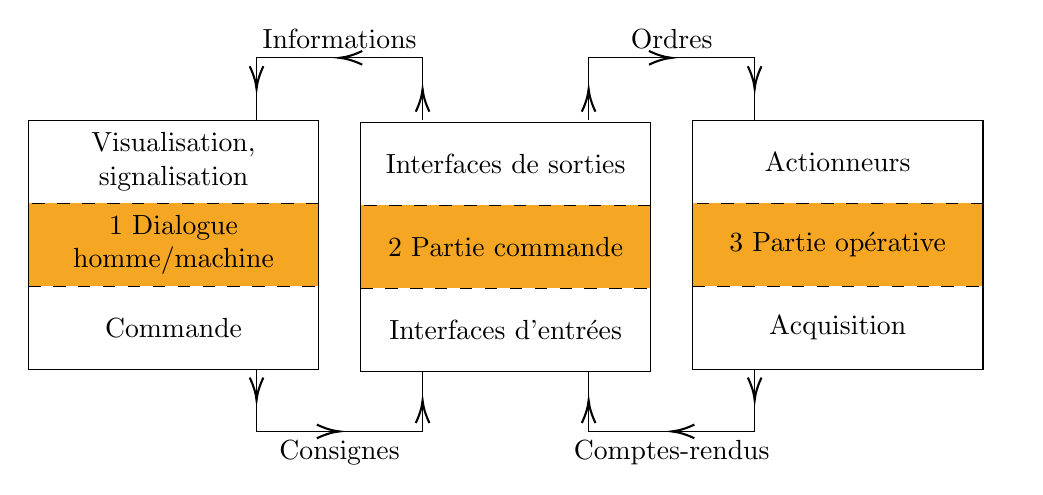
\begin{tikzpicture}[x=0.75pt,y=0.75pt,yscale=-1,xscale=1]
%uncomment if require: \path (0,300); %set diagram left start at 0, and has height of 300

%Shape: Rectangle [id:dp10260270003045247] 
\draw  [fill={rgb, 255:red, 245; green, 166; blue, 35 }  ,fill opacity=1 ] (100,90) -- (240,90) -- (240,210) -- (100,210) -- cycle ;
%Shape: Rectangle [id:dp6595603315617775] 
\draw  [fill={rgb, 255:red, 255; green, 255; blue, 255 }  ,fill opacity=1 ][dash pattern={on 4.5pt off 4.5pt}] (100,90) -- (240,90) -- (240,130) -- (100,130) -- cycle ;
%Shape: Rectangle [id:dp9769956373140513] 
\draw  [fill={rgb, 255:red, 255; green, 255; blue, 255 }  ,fill opacity=1 ][dash pattern={on 4.5pt off 4.5pt}] (100,170) -- (240,170) -- (240,210) -- (100,210) -- cycle ;
%Shape: Rectangle [id:dp5049152868754619] 
\draw  [fill={rgb, 255:red, 245; green, 166; blue, 35 }  ,fill opacity=1 ] (260,91) -- (400,91) -- (400,211) -- (260,211) -- cycle ;
%Shape: Rectangle [id:dp9221854973091113] 
\draw  [fill={rgb, 255:red, 245; green, 166; blue, 35 }  ,fill opacity=1 ] (420,90) -- (560,90) -- (560,210) -- (420,210) -- cycle ;
%Straight Lines [id:da1386624660715703] 
\draw    (210,90) -- (210,60) -- (290,60) -- (290,90) ;
\draw [shift={(210,75)}, rotate = 270] [color={rgb, 255:red, 0; green, 0; blue, 0 }  ][line width=0.75]    (10.93,-3.29) .. controls (6.95,-1.4) and (3.31,-0.3) .. (0,0) .. controls (3.31,0.3) and (6.95,1.4) .. (10.93,3.29)   ;
\draw [shift={(250,60)}, rotate = 0] [color={rgb, 255:red, 0; green, 0; blue, 0 }  ][line width=0.75]    (10.93,-3.29) .. controls (6.95,-1.4) and (3.31,-0.3) .. (0,0) .. controls (3.31,0.3) and (6.95,1.4) .. (10.93,3.29)   ;
\draw [shift={(290,75)}, rotate = 90] [color={rgb, 255:red, 0; green, 0; blue, 0 }  ][line width=0.75]    (10.93,-3.29) .. controls (6.95,-1.4) and (3.31,-0.3) .. (0,0) .. controls (3.31,0.3) and (6.95,1.4) .. (10.93,3.29)   ;
%Straight Lines [id:da24586017428466933] 
\draw    (210,210) -- (210,240) -- (290,240) -- (290,210) ;
\draw [shift={(210,225)}, rotate = 270] [color={rgb, 255:red, 0; green, 0; blue, 0 }  ][line width=0.75]    (10.93,-3.29) .. controls (6.95,-1.4) and (3.31,-0.3) .. (0,0) .. controls (3.31,0.3) and (6.95,1.4) .. (10.93,3.29)   ;
\draw [shift={(250,240)}, rotate = 180] [color={rgb, 255:red, 0; green, 0; blue, 0 }  ][line width=0.75]    (10.93,-3.29) .. controls (6.95,-1.4) and (3.31,-0.3) .. (0,0) .. controls (3.31,0.3) and (6.95,1.4) .. (10.93,3.29)   ;
\draw [shift={(290,225)}, rotate = 450] [color={rgb, 255:red, 0; green, 0; blue, 0 }  ][line width=0.75]    (10.93,-3.29) .. controls (6.95,-1.4) and (3.31,-0.3) .. (0,0) .. controls (3.31,0.3) and (6.95,1.4) .. (10.93,3.29)   ;
%Straight Lines [id:da47558842927164535] 
\draw    (370,90) -- (370,60) -- (450,60) -- (450,90) ;
\draw [shift={(370,75)}, rotate = 450] [color={rgb, 255:red, 0; green, 0; blue, 0 }  ][line width=0.75]    (10.93,-3.29) .. controls (6.95,-1.4) and (3.31,-0.3) .. (0,0) .. controls (3.31,0.3) and (6.95,1.4) .. (10.93,3.29)   ;
\draw [shift={(410,60)}, rotate = 180] [color={rgb, 255:red, 0; green, 0; blue, 0 }  ][line width=0.75]    (10.93,-3.29) .. controls (6.95,-1.4) and (3.31,-0.3) .. (0,0) .. controls (3.31,0.3) and (6.95,1.4) .. (10.93,3.29)   ;
\draw [shift={(450,75)}, rotate = 270] [color={rgb, 255:red, 0; green, 0; blue, 0 }  ][line width=0.75]    (10.93,-3.29) .. controls (6.95,-1.4) and (3.31,-0.3) .. (0,0) .. controls (3.31,0.3) and (6.95,1.4) .. (10.93,3.29)   ;
%Straight Lines [id:da04414261859625401] 
\draw    (370,210) -- (370,240) -- (450,240) -- (450,210) ;
\draw [shift={(370,225)}, rotate = 90] [color={rgb, 255:red, 0; green, 0; blue, 0 }  ][line width=0.75]    (10.93,-3.29) .. controls (6.95,-1.4) and (3.31,-0.3) .. (0,0) .. controls (3.31,0.3) and (6.95,1.4) .. (10.93,3.29)   ;
\draw [shift={(410,240)}, rotate = 0] [color={rgb, 255:red, 0; green, 0; blue, 0 }  ][line width=0.75]    (10.93,-3.29) .. controls (6.95,-1.4) and (3.31,-0.3) .. (0,0) .. controls (3.31,0.3) and (6.95,1.4) .. (10.93,3.29)   ;
\draw [shift={(450,225)}, rotate = 270] [color={rgb, 255:red, 0; green, 0; blue, 0 }  ][line width=0.75]    (10.93,-3.29) .. controls (6.95,-1.4) and (3.31,-0.3) .. (0,0) .. controls (3.31,0.3) and (6.95,1.4) .. (10.93,3.29)   ;
%Shape: Rectangle [id:dp23929095996485295] 
\draw  [fill={rgb, 255:red, 255; green, 255; blue, 255 }  ,fill opacity=1 ][dash pattern={on 4.5pt off 4.5pt}] (260,91) -- (400,91) -- (400,131) -- (260,131) -- cycle ;
%Shape: Rectangle [id:dp2763405581796431] 
\draw  [fill={rgb, 255:red, 255; green, 255; blue, 255 }  ,fill opacity=1 ][dash pattern={on 4.5pt off 4.5pt}] (260,171) -- (400,171) -- (400,211) -- (260,211) -- cycle ;
%Shape: Rectangle [id:dp7537953936366432] 
\draw  [fill={rgb, 255:red, 255; green, 255; blue, 255 }  ,fill opacity=1 ][dash pattern={on 4.5pt off 4.5pt}] (420,90) -- (560,90) -- (560,130) -- (420,130) -- cycle ;
%Shape: Rectangle [id:dp8221584429330733] 
\draw  [fill={rgb, 255:red, 255; green, 255; blue, 255 }  ,fill opacity=1 ][dash pattern={on 4.5pt off 4.5pt}] (420,170) -- (560,170) -- (560,210) -- (420,210) -- cycle ;
%Shape: Rectangle [id:dp7256077006177953] 
\draw   (100,90) -- (240,90) -- (240,210) -- (100,210) -- cycle ;
%Shape: Rectangle [id:dp09975149655953441] 
\draw   (260,91) -- (400,91) -- (400,211) -- (260,211) -- cycle ;
%Shape: Rectangle [id:dp8308335059986585] 
\draw   (420,90) -- (560,90) -- (560,210) -- (420,210) -- cycle ;

% Text Node
\draw (170,110) node   [align=left] {\begin{minipage}[lt]{65.47125pt}\setlength\topsep{0pt}
\begin{center}
Visualisation, \\signalisation
\end{center}

\end{minipage}};
% Text Node
\draw (170,150) node   [align=left] {\begin{minipage}[lt]{92.88375pt}\setlength\topsep{0pt}
\begin{center}
\Circled{1} Dialogue \\homme/machine
\end{center}

\end{minipage}};
% Text Node
\draw (170,190) node   [align=left] {\begin{minipage}[lt]{55.451875pt}\setlength\topsep{0pt}
\begin{center}
Commande
\end{center}

\end{minipage}};
% Text Node
\draw (330,111) node   [align=left] {\begin{minipage}[lt]{94.573125pt}\setlength\topsep{0pt}
\begin{center}
Interfaces de sorties
\end{center}

\end{minipage}};
% Text Node
\draw (330,151) node   [align=left] {\begin{minipage}[lt]{129.720625pt}\setlength\topsep{0pt}
\begin{center}
\Circled{2} Partie commande
\end{center}

\end{minipage}};
% Text Node
\draw (330,191) node   [align=left] {\begin{minipage}[lt]{91.99125000000001pt}\setlength\topsep{0pt}
\begin{center}
Interfaces d'entrées
\end{center}

\end{minipage}};
% Text Node
\draw (490,110) node   [align=left] {\begin{minipage}[lt]{56.588750000000005pt}\setlength\topsep{0pt}
\begin{center}
Actionneurs
\end{center}

\end{minipage}};
% Text Node
\draw (490,150) node   [align=left] {\begin{minipage}[lt]{121.22062500000001pt}\setlength\topsep{0pt}
\begin{center}
\Circled{3} Partie opérative
\end{center}

\end{minipage}};
% Text Node
\draw (490,190) node   [align=left] {\begin{minipage}[lt]{52.051875pt}\setlength\topsep{0pt}
\begin{center}
Acquisition
\end{center}

\end{minipage}};
% Text Node
\draw (250,57) node [anchor=south] [inner sep=0.75pt]   [align=left] {Informations};
% Text Node
\draw (410,57) node [anchor=south] [inner sep=0.75pt]   [align=left] {Ordres};
% Text Node
\draw (410,243) node [anchor=north] [inner sep=0.75pt]   [align=left] {Comptes-rendus};
% Text Node
\draw (250,243) node [anchor=north] [inner sep=0.75pt]   [align=left] {Consignes};


\end{tikzpicture}
\end{figure}
%\end{document}



\begin{definition}{Dialogue homme-machine}{}
Cette partie permet le dialogue entre l'opérateur et la partie commande. L'opérateur envoie des \emph{consignes opérateurs} et reçoit des \emph{informations visuelles}.
Les consignes opérateurs permettent à l'opérateur de donner des ordres d'exécution à la partie commande et les informations visuelles permettent à l'opérateur de suivre la production.
\end{definition}

\begin{definition}{Partie commande}{}
La partie commande élabore les \emph{consignes opératives} à partir des \emph{consignes opérateurs}, des \emph{compte-rendus} des capteurs et du programme intégré. Les consignes opératives correspondent aux ordres que la partie commande donne à la partie opérative et les compte-rendus, élaborés par les différents capteurs placés sur la partie opérative, informent la partie commande de la bonne exécution des ordres envoyés.
\end{definition}

\begin{definition}{Partie opérative}{}
La partie opérative assure la transformation de la \emph{matière d'\oe{}uvre}.
\end{definition}

\subsection{Structure fonctionnelle d'un système automatisé}

\begin{definition}{Structure fonctionnelle d'un système automatisé}{}
Un \emph{système technique} peut être considéré comme la coordination d'une \emph{chaine d'acquisition} et d'une \emph{chaine d'énergie}, comportant chacune des fonctions propres.
\end{definition}

%--------------------------------------
%CANEVAS
%--------------------------------------

%utiliser les environnement \begin{comment} \end{comment} pour mettre en commentaire le préambule une fois la programmation appelée dans le document maître (!ne pas oublier de mettre en commentaire \end{document}!)

\begin{comment}

\documentclass[a4paper, 11pt, twoside, fleqn]{memoir}

\usepackage{AOCDTF}

\marqueurchapitre
\decoupagechapitre{1} %juste pour éviter les erreurs lors de la compilation des sous-programmations (passera en commentaire)

%lien d'édition des figures Tikz sur le site mathcha.io (rajouter le lien d'une modification effectuée sur la figure tikz avec le nom du modificateur car il n'y a qu'un lien par compte)

%lien mathcha Nom Prénom : https://www.mathcha.io/editor/ml76PuOwsvWh8WD77ytO3OJn2Hlvq8GNF3g2Jwd

%--------------------------------------
%corps du document
%--------------------------------------

\begin{document} %corps du document
	\openleft %début de chapitre à gauche

\end{comment}

\begin{figure}[H]
\caption{Structure fonctionnelle d'un système automatisé}



\tikzset{every picture/.style={line width=0.75pt}} %set default line width to 0.75pt        

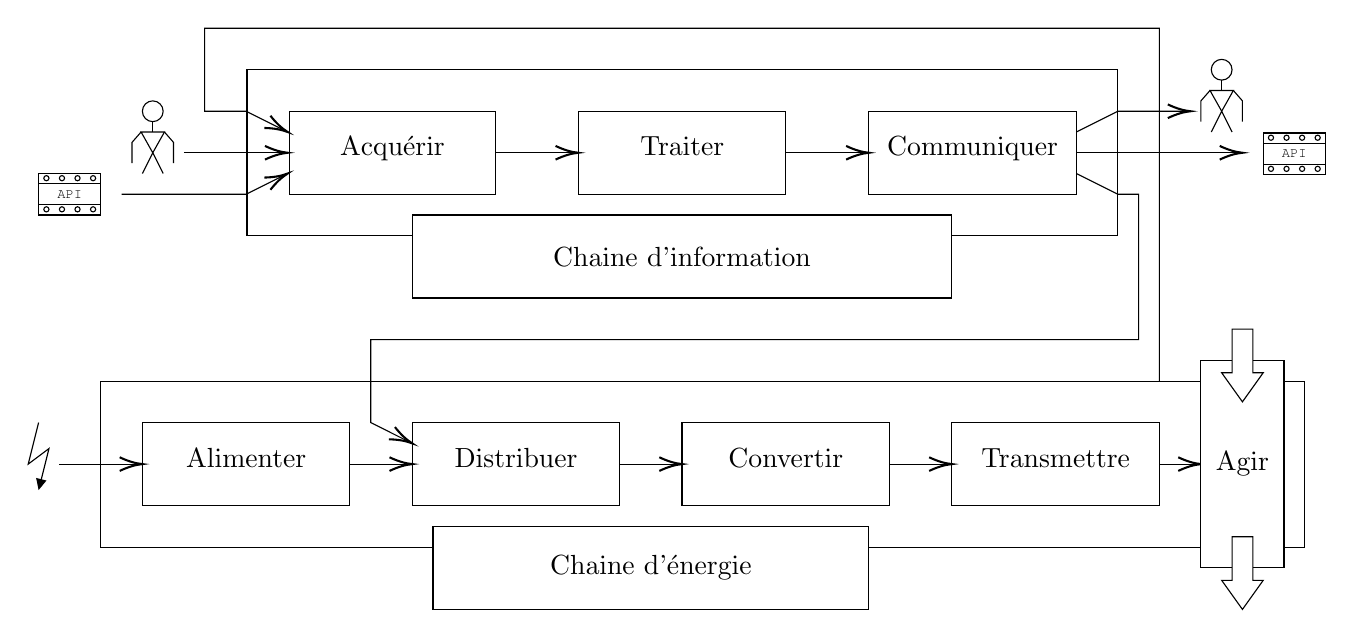
\begin{tikzpicture}[x=0.75pt,y=0.75pt,yscale=-1,xscale=1]
%uncomment if require: \path (0,300); %set diagram left start at 0, and has height of 300

%Shape: Rectangle [id:dp8447559891320054] 
\draw   (141,50) -- (240,50) -- (240,90) -- (141,90) -- cycle ;
%Shape: Rectangle [id:dp5040395055749388] 
\draw   (120.38,30) -- (539.88,30) -- (539.88,110) -- (120.38,110) -- cycle ;
%Shape: Rectangle [id:dp3485755093258376] 
\draw   (420,50) -- (520,50) -- (520,90) -- (420,90) -- cycle ;
%Straight Lines [id:da13944803821905194] 
\draw    (60,90) -- (120,90) -- (138.21,80.89) ;
\draw [shift={(140,80)}, rotate = 513.4300000000001] [color={rgb, 255:red, 0; green, 0; blue, 0 }  ][line width=0.75]    (10.93,-3.29) .. controls (6.95,-1.4) and (3.31,-0.3) .. (0,0) .. controls (3.31,0.3) and (6.95,1.4) .. (10.93,3.29)   ;
%Straight Lines [id:da7480256316518205] 
\draw    (90,70) -- (138,70) ;
\draw [shift={(140,70)}, rotate = 180] [color={rgb, 255:red, 0; green, 0; blue, 0 }  ][line width=0.75]    (10.93,-3.29) .. controls (6.95,-1.4) and (3.31,-0.3) .. (0,0) .. controls (3.31,0.3) and (6.95,1.4) .. (10.93,3.29)   ;
%Straight Lines [id:da6039515419453989] 
\draw    (560,180) -- (560,10) -- (100,10) -- (100,50) -- (120,50) -- (138.21,59.11) ;
\draw [shift={(140,60)}, rotate = 206.57] [color={rgb, 255:red, 0; green, 0; blue, 0 }  ][line width=0.75]    (10.93,-3.29) .. controls (6.95,-1.4) and (3.31,-0.3) .. (0,0) .. controls (3.31,0.3) and (6.95,1.4) .. (10.93,3.29)   ;
%Shape: Rectangle [id:dp9681113408051312] 
\draw  [fill={rgb, 255:red, 255; green, 255; blue, 255 }  ,fill opacity=1 ] (200,100) -- (460,100) -- (460,140) -- (200,140) -- cycle ;
%Straight Lines [id:da6666559084323214] 
\draw    (70,80) -- (75,70) -- (80,80) ;
%Shape: Triangle [id:dp8670605189789042] 
\draw   (75,70) -- (80.63,60) -- (69.38,60) -- cycle ;
%Straight Lines [id:da2128171133282747] 
\draw    (80.63,60) -- (85,65) -- (85,75) ;
%Straight Lines [id:da048501017255865975] 
\draw    (69.38,60) -- (65,65) -- (65,75) ;
%Straight Lines [id:da9159576451370222] 
\draw    (75,55) -- (75,60) ;
%Shape: Circle [id:dp5959447127284796] 
\draw   (70,50) .. controls (70,47.24) and (72.24,45) .. (75,45) .. controls (77.76,45) and (80,47.24) .. (80,50) .. controls (80,52.76) and (77.76,55) .. (75,55) .. controls (72.24,55) and (70,52.76) .. (70,50) -- cycle ;
%Shape: Rectangle [id:dp055554891197074796] 
\draw   (20,80) -- (50,80) -- (50,100) -- (20,100) -- cycle ;
%Shape: Rectangle [id:dp9603377302842956] 
\draw   (20,80) -- (50,80) -- (50,85) -- (20,85) -- cycle ;
%Shape: Circle [id:dp1096340469284306] 
\draw   (22.5,82.25) .. controls (22.5,81.56) and (23.06,81) .. (23.75,81) .. controls (24.44,81) and (25,81.56) .. (25,82.25) .. controls (25,82.94) and (24.44,83.5) .. (23.75,83.5) .. controls (23.06,83.5) and (22.5,82.94) .. (22.5,82.25) -- cycle ;
%Shape: Circle [id:dp8181510182873335] 
\draw   (30,82.25) .. controls (30,81.56) and (30.56,81) .. (31.25,81) .. controls (31.94,81) and (32.5,81.56) .. (32.5,82.25) .. controls (32.5,82.94) and (31.94,83.5) .. (31.25,83.5) .. controls (30.56,83.5) and (30,82.94) .. (30,82.25) -- cycle ;
%Shape: Circle [id:dp18832963357311028] 
\draw   (37.5,82.25) .. controls (37.5,81.56) and (38.06,81) .. (38.75,81) .. controls (39.44,81) and (40,81.56) .. (40,82.25) .. controls (40,82.94) and (39.44,83.5) .. (38.75,83.5) .. controls (38.06,83.5) and (37.5,82.94) .. (37.5,82.25) -- cycle ;
%Shape: Circle [id:dp07795180108476385] 
\draw   (45,82.25) .. controls (45,81.56) and (45.56,81) .. (46.25,81) .. controls (46.94,81) and (47.5,81.56) .. (47.5,82.25) .. controls (47.5,82.94) and (46.94,83.5) .. (46.25,83.5) .. controls (45.56,83.5) and (45,82.94) .. (45,82.25) -- cycle ;
%Shape: Rectangle [id:dp8193392068369237] 
\draw   (20,95) -- (50,95) -- (50,100) -- (20,100) -- cycle ;
%Shape: Circle [id:dp8865059600085532] 
\draw   (22.5,97.25) .. controls (22.5,96.56) and (23.06,96) .. (23.75,96) .. controls (24.44,96) and (25,96.56) .. (25,97.25) .. controls (25,97.94) and (24.44,98.5) .. (23.75,98.5) .. controls (23.06,98.5) and (22.5,97.94) .. (22.5,97.25) -- cycle ;
%Shape: Circle [id:dp8454673451628865] 
\draw   (30,97.25) .. controls (30,96.56) and (30.56,96) .. (31.25,96) .. controls (31.94,96) and (32.5,96.56) .. (32.5,97.25) .. controls (32.5,97.94) and (31.94,98.5) .. (31.25,98.5) .. controls (30.56,98.5) and (30,97.94) .. (30,97.25) -- cycle ;
%Shape: Circle [id:dp5548349291344336] 
\draw   (37.5,97.25) .. controls (37.5,96.56) and (38.06,96) .. (38.75,96) .. controls (39.44,96) and (40,96.56) .. (40,97.25) .. controls (40,97.94) and (39.44,98.5) .. (38.75,98.5) .. controls (38.06,98.5) and (37.5,97.94) .. (37.5,97.25) -- cycle ;
%Shape: Circle [id:dp030251697162806623] 
\draw   (45,97.25) .. controls (45,96.56) and (45.56,96) .. (46.25,96) .. controls (46.94,96) and (47.5,96.56) .. (47.5,97.25) .. controls (47.5,97.94) and (46.94,98.5) .. (46.25,98.5) .. controls (45.56,98.5) and (45,97.94) .. (45,97.25) -- cycle ;
%Straight Lines [id:da8688770925382665] 
\draw    (585,60) -- (590,50) -- (595,60) ;
%Shape: Triangle [id:dp6554661457263661] 
\draw   (590,50) -- (595.63,40) -- (584.38,40) -- cycle ;
%Straight Lines [id:da739342857188235] 
\draw    (595.63,40) -- (600,45) -- (600,55) ;
%Straight Lines [id:da540156258084405] 
\draw    (584.38,40) -- (580,45) -- (580,55) ;
%Straight Lines [id:da14442018464243855] 
\draw    (590,35) -- (590,40) ;
%Shape: Circle [id:dp494511824746114] 
\draw   (585,30) .. controls (585,27.24) and (587.24,25) .. (590,25) .. controls (592.76,25) and (595,27.24) .. (595,30) .. controls (595,32.76) and (592.76,35) .. (590,35) .. controls (587.24,35) and (585,32.76) .. (585,30) -- cycle ;
%Straight Lines [id:da7486849017599221] 
\draw    (520,60) -- (540,50) -- (573,50) ;
\draw [shift={(575,50)}, rotate = 180] [color={rgb, 255:red, 0; green, 0; blue, 0 }  ][line width=0.75]    (10.93,-3.29) .. controls (6.95,-1.4) and (3.31,-0.3) .. (0,0) .. controls (3.31,0.3) and (6.95,1.4) .. (10.93,3.29)   ;
%Straight Lines [id:da5179214989239102] 
\draw    (520,70) -- (598,70) ;
\draw [shift={(600,70)}, rotate = 180] [color={rgb, 255:red, 0; green, 0; blue, 0 }  ][line width=0.75]    (10.93,-3.29) .. controls (6.95,-1.4) and (3.31,-0.3) .. (0,0) .. controls (3.31,0.3) and (6.95,1.4) .. (10.93,3.29)   ;
%Shape: Rectangle [id:dp2676559271683636] 
\draw   (610,60.5) -- (640,60.5) -- (640,80.5) -- (610,80.5) -- cycle ;
%Shape: Rectangle [id:dp42727858879338465] 
\draw   (610,60.5) -- (640,60.5) -- (640,65.5) -- (610,65.5) -- cycle ;
%Shape: Circle [id:dp7450655459966928] 
\draw   (612.5,62.75) .. controls (612.5,62.06) and (613.06,61.5) .. (613.75,61.5) .. controls (614.44,61.5) and (615,62.06) .. (615,62.75) .. controls (615,63.44) and (614.44,64) .. (613.75,64) .. controls (613.06,64) and (612.5,63.44) .. (612.5,62.75) -- cycle ;
%Shape: Circle [id:dp7953756563963081] 
\draw   (620,62.75) .. controls (620,62.06) and (620.56,61.5) .. (621.25,61.5) .. controls (621.94,61.5) and (622.5,62.06) .. (622.5,62.75) .. controls (622.5,63.44) and (621.94,64) .. (621.25,64) .. controls (620.56,64) and (620,63.44) .. (620,62.75) -- cycle ;
%Shape: Circle [id:dp2507045704894587] 
\draw   (627.5,62.75) .. controls (627.5,62.06) and (628.06,61.5) .. (628.75,61.5) .. controls (629.44,61.5) and (630,62.06) .. (630,62.75) .. controls (630,63.44) and (629.44,64) .. (628.75,64) .. controls (628.06,64) and (627.5,63.44) .. (627.5,62.75) -- cycle ;
%Shape: Circle [id:dp5498495085183052] 
\draw   (635,62.75) .. controls (635,62.06) and (635.56,61.5) .. (636.25,61.5) .. controls (636.94,61.5) and (637.5,62.06) .. (637.5,62.75) .. controls (637.5,63.44) and (636.94,64) .. (636.25,64) .. controls (635.56,64) and (635,63.44) .. (635,62.75) -- cycle ;
%Shape: Rectangle [id:dp6783546198133718] 
\draw   (610,75.5) -- (640,75.5) -- (640,80.5) -- (610,80.5) -- cycle ;
%Shape: Circle [id:dp037195434851017395] 
\draw   (612.5,77.75) .. controls (612.5,77.06) and (613.06,76.5) .. (613.75,76.5) .. controls (614.44,76.5) and (615,77.06) .. (615,77.75) .. controls (615,78.44) and (614.44,79) .. (613.75,79) .. controls (613.06,79) and (612.5,78.44) .. (612.5,77.75) -- cycle ;
%Shape: Circle [id:dp37951251473058556] 
\draw   (620,77.75) .. controls (620,77.06) and (620.56,76.5) .. (621.25,76.5) .. controls (621.94,76.5) and (622.5,77.06) .. (622.5,77.75) .. controls (622.5,78.44) and (621.94,79) .. (621.25,79) .. controls (620.56,79) and (620,78.44) .. (620,77.75) -- cycle ;
%Shape: Circle [id:dp42318982954941686] 
\draw   (627.5,77.75) .. controls (627.5,77.06) and (628.06,76.5) .. (628.75,76.5) .. controls (629.44,76.5) and (630,77.06) .. (630,77.75) .. controls (630,78.44) and (629.44,79) .. (628.75,79) .. controls (628.06,79) and (627.5,78.44) .. (627.5,77.75) -- cycle ;
%Shape: Circle [id:dp7706743761911097] 
\draw   (635,77.75) .. controls (635,77.06) and (635.56,76.5) .. (636.25,76.5) .. controls (636.94,76.5) and (637.5,77.06) .. (637.5,77.75) .. controls (637.5,78.44) and (636.94,79) .. (636.25,79) .. controls (635.56,79) and (635,78.44) .. (635,77.75) -- cycle ;
%Straight Lines [id:da6480566883244047] 
\draw    (520,80) -- (540,90) -- (550,90) -- (550,160) -- (180,160) -- (180,200) -- (198.21,209.11) ;
\draw [shift={(200,210)}, rotate = 206.57] [color={rgb, 255:red, 0; green, 0; blue, 0 }  ][line width=0.75]    (10.93,-3.29) .. controls (6.95,-1.4) and (3.31,-0.3) .. (0,0) .. controls (3.31,0.3) and (6.95,1.4) .. (10.93,3.29)   ;
%Straight Lines [id:da741578299811131] 
\draw    (240,70) -- (278,70) ;
\draw [shift={(280,70)}, rotate = 180] [color={rgb, 255:red, 0; green, 0; blue, 0 }  ][line width=0.75]    (10.93,-3.29) .. controls (6.95,-1.4) and (3.31,-0.3) .. (0,0) .. controls (3.31,0.3) and (6.95,1.4) .. (10.93,3.29)   ;
%Straight Lines [id:da9578943679426587] 
\draw    (380,70) -- (418,70) ;
\draw [shift={(420,70)}, rotate = 180] [color={rgb, 255:red, 0; green, 0; blue, 0 }  ][line width=0.75]    (10.93,-3.29) .. controls (6.95,-1.4) and (3.31,-0.3) .. (0,0) .. controls (3.31,0.3) and (6.95,1.4) .. (10.93,3.29)   ;
%Shape: Rectangle [id:dp7625531172106348] 
\draw   (50,180) -- (630,180) -- (630,260) -- (50,260) -- cycle ;
%Straight Lines [id:da06518814932367034] 
\draw    (30,220) -- (68,220) ;
\draw [shift={(70,220)}, rotate = 180] [color={rgb, 255:red, 0; green, 0; blue, 0 }  ][line width=0.75]    (10.93,-3.29) .. controls (6.95,-1.4) and (3.31,-0.3) .. (0,0) .. controls (3.31,0.3) and (6.95,1.4) .. (10.93,3.29)   ;
%Straight Lines [id:da05820201299681205] 
\draw    (20,200) -- (15,220) -- (25,212.5) -- (20.73,229.59) ;
\draw [shift={(20,232.5)}, rotate = 284.04] [fill={rgb, 255:red, 0; green, 0; blue, 0 }  ][line width=0.08]  [draw opacity=0] (5.36,-2.57) -- (0,0) -- (5.36,2.57) -- cycle    ;
%Shape: Rectangle [id:dp10434084261428833] 
\draw   (70,200) -- (170,200) -- (170,240) -- (70,240) -- cycle ;
%Shape: Rectangle [id:dp18606228570622307] 
\draw   (200,200) -- (300,200) -- (300,240) -- (200,240) -- cycle ;
%Shape: Rectangle [id:dp7841045741615225] 
\draw   (330,200) -- (430,200) -- (430,240) -- (330,240) -- cycle ;
%Straight Lines [id:da55269288534927] 
\draw    (170,220) -- (198,220) ;
\draw [shift={(200,220)}, rotate = 180] [color={rgb, 255:red, 0; green, 0; blue, 0 }  ][line width=0.75]    (10.93,-3.29) .. controls (6.95,-1.4) and (3.31,-0.3) .. (0,0) .. controls (3.31,0.3) and (6.95,1.4) .. (10.93,3.29)   ;
%Shape: Rectangle [id:dp2727970736301596] 
\draw   (460,200) -- (560,200) -- (560,240) -- (460,240) -- cycle ;
%Shape: Rectangle [id:dp9496735175137397] 
\draw  [fill={rgb, 255:red, 255; green, 255; blue, 255 }  ,fill opacity=1 ] (210,250) -- (420,250) -- (420,290) -- (210,290) -- cycle ;
%Straight Lines [id:da39218931857608086] 
\draw    (300,220) -- (328,220) ;
\draw [shift={(330,220)}, rotate = 180] [color={rgb, 255:red, 0; green, 0; blue, 0 }  ][line width=0.75]    (10.93,-3.29) .. controls (6.95,-1.4) and (3.31,-0.3) .. (0,0) .. controls (3.31,0.3) and (6.95,1.4) .. (10.93,3.29)   ;
%Straight Lines [id:da044626104039806824] 
\draw    (430,220) -- (458,220) ;
\draw [shift={(460,220)}, rotate = 180] [color={rgb, 255:red, 0; green, 0; blue, 0 }  ][line width=0.75]    (10.93,-3.29) .. controls (6.95,-1.4) and (3.31,-0.3) .. (0,0) .. controls (3.31,0.3) and (6.95,1.4) .. (10.93,3.29)   ;
%Straight Lines [id:da8845694742729966] 
\draw    (560,220) -- (578,220) ;
\draw [shift={(580,220)}, rotate = 180] [color={rgb, 255:red, 0; green, 0; blue, 0 }  ][line width=0.75]    (10.93,-3.29) .. controls (6.95,-1.4) and (3.31,-0.3) .. (0,0) .. controls (3.31,0.3) and (6.95,1.4) .. (10.93,3.29)   ;
%Shape: Rectangle [id:dp15077484556954057] 
\draw  [fill={rgb, 255:red, 255; green, 255; blue, 255 }  ,fill opacity=1 ] (580,170) -- (620,170) -- (620,270) -- (580,270) -- cycle ;
%Right Arrow [id:dp5753618254098206] 
\draw  [fill={rgb, 255:red, 255; green, 255; blue, 255 }  ,fill opacity=1 ] (605,155) -- (605,176) -- (610,176) -- (600,190) -- (590,176) -- (595,176) -- (595,155) -- cycle ;
%Right Arrow [id:dp9867249038172623] 
\draw  [fill={rgb, 255:red, 255; green, 255; blue, 255 }  ,fill opacity=1 ] (605,255) -- (605,276) -- (610,276) -- (600,290) -- (590,276) -- (595,276) -- (595,255) -- cycle ;
%Shape: Rectangle [id:dp5178391173237168] 
\draw   (280.25,50) -- (380,50) -- (380,90) -- (280.25,90) -- cycle ;

% Text Node
\draw (190.5,68) node  [font=\normalsize] [align=left] {\begin{minipage}[lt]{40.704375000000006pt}\setlength\topsep{0pt}
\begin{center}
Acquérir
\end{center}

\end{minipage}};
% Text Node
\draw (470,68) node  [font=\normalsize] [align=left] {\begin{minipage}[lt]{66.78875000000001pt}\setlength\topsep{0pt}
\begin{center}
Communiquer
\end{center}

\end{minipage}};
% Text Node
\draw (330,120) node  [font=\normalsize] [align=left] {\begin{minipage}[lt]{95.95437500000001pt}\setlength\topsep{0pt}
\begin{center}
Chaine d'information
\end{center}

\end{minipage}};
% Text Node
\draw (35,90) node   [align=left] {{\tiny {\fontfamily{pcr}\selectfont API}}};
% Text Node
\draw (625,70.5) node   [align=left] {{\tiny {\fontfamily{pcr}\selectfont API}}};
% Text Node
\draw (120,217) node  [font=\normalsize] [align=left] {\begin{minipage}[lt]{45.804375pt}\setlength\topsep{0pt}
\begin{center}
Alimenter
\end{center}

\end{minipage}};
% Text Node
\draw (250,217) node  [font=\normalsize] [align=left] {\begin{minipage}[lt]{46.36750000000001pt}\setlength\topsep{0pt}
\begin{center}
Distribuer
\end{center}

\end{minipage}};
% Text Node
\draw (380,217) node  [font=\normalsize] [align=left] {\begin{minipage}[lt]{44.104375000000005pt}\setlength\topsep{0pt}
\begin{center}
Convertir
\end{center}

\end{minipage}};
% Text Node
\draw (510,217) node  [font=\normalsize] [align=left] {\begin{minipage}[lt]{57.321875000000006pt}\setlength\topsep{0pt}
\begin{center}
Transmettre
\end{center}

\end{minipage}};
% Text Node
\draw (315,270) node  [font=\normalsize] [align=left] {\begin{minipage}[lt]{79.528125pt}\setlength\topsep{0pt}
\begin{center}
Chaine d'énergie
\end{center}

\end{minipage}};
% Text Node
\draw (600,220) node  [font=\normalsize] [align=left] {\begin{minipage}[lt]{20.867500000000003pt}\setlength\topsep{0pt}
\begin{center}
Agir
\end{center}

\end{minipage}};
% Text Node
\draw (330.13,67) node  [font=\normalsize] [align=left] {\begin{minipage}[lt]{31.81125pt}\setlength\topsep{0pt}
\begin{center}
Traiter
\end{center}

\end{minipage}};


\end{tikzpicture}






\end{figure}



%\end{document}






Les fonctions techniques régissant ces chaines sont les suivantes :
\begin{description}
\item [Chaine d'information :] regroupement de tous les organes de prélèvement, de traitement et de communication des informations, dont la chaîne d'acquisition est l'un des éléments\,;
	\begin{description}
	\item [Acquérir :] premier élément de la chaine d'information qui permet le prélèvement des informations par l'intermédiaire de capteurs et d'autres systèmes d'acquisition. Ces informations proviennent de trois parties du système technique :
		\begin{description}
		\item [Informations provenant d'un autre système :] organes de traitement et parties commandes pouvant échanger des informations et des ressources lorsqu'ils sont interconnectés en réseau\,;
		\item [Informations provenant de l'utilisateur :] transmission par l'utilisateur du système d'informations et consignes au système, par l'intermédiaire d'un clavier ou d'éléments du pupitre de dialogue\,;
		\item [Grandeurs physiques à acquérir :] transmission d'informations d'état du système par des \emph{capteurs} placés sur la chaine d'énergie\,;
		\end{description}
	\item [Traiter :] organe de traitement de l'information prénommé \emph{partie commande}, s'agissant presqu'exclusivement de systèmes électroniques (programmables ou non)\,;
		\begin{description}
		\item []
		\end{description}
	\end{description}
\end{description}







%\end{document}

